\newpage
\section{Lineare Algebra}
\subsection{Eigenwerte / Eigenvektoren}
\textbf{Eigenwerte}: $det(A-\lambda E) = 0$ lösen\\

\textbf{Eigenvektoren}: $(A-\lambda_i E)v = 0$ lösen\\

\textbf{Inverse 2x2-Matrizen}\\
$A^{-1} = \begin{bmatrix}
a & b \\ c & d \\
\end{bmatrix}^{-1} =
\frac{1}{\det(A)} \begin{bmatrix}
d & -b \\ -c & a \\
\end{bmatrix}  =
\frac{1}{ad-bc} \begin{bmatrix}
d & -b \\ -c & a \\
\end{bmatrix}$

\textbf{Inverse 3x3-Matrizen}\\
$A^{-1} = \begin{bmatrix}
a & b & c\\ d & e & f \\ g & h & i \\
\end{bmatrix}^{-1} =
\frac{1}{\det(A)} \begin{bmatrix}
ei - fh & ch - bi & bf - ce \\
fg - di & ai - cg & cd - af \\
dh - eg & bg - ah & ae - bd
\end{bmatrix}$

\textbf{Determinante}

$2 \times 2$-Matrix:
$\det
 \begin{bmatrix}
 a_{11} & a_{12} \\
 a_{21} & a_{22}
 \end{bmatrix}
= a_{11} a_{22} - a_{12} a_{21}$

$3 \times 3$-Matrix:
$\det
 \begin{bmatrix}
 a_{11} & a_{12} & a_{13} \\
 a_{21} & a_{22} & a_{23} \\
 a_{31} & a_{32} & a_{33}
 \end{bmatrix} = a_{11} a_{22} a_{33} +a_{12} a_{23} a_{31} + a_{13} a_{21} a_{32} - a_{13} a_{22} a_{31} - a_{12} a_{21} a_{33} - a_{11} a_{23} a_{32}$

\textbf{Laplacescher Entwicklungssatz}

Mit dem Laplaceschen Entwicklungssatz kann man die Determinante einer $n \times n$-Matrix „nach einer Zeile oder Spalte entwickeln“. Die beiden Formeln lauten:\\
$\det A = \sum_{i=1}^n (-1)^{i+j} \cdot a_{ij} \cdot \det A_{ij}$ (Entwicklung nach der $j$-ten Spalte)\\
$\det A = \sum_{j=1}^n (-1)^{i+j} \cdot a_{ij} \cdot \det A_{ij}$ (Entwicklung nach der $i$-ten Zeile)\\
wobei $A_{ij}$ die $(n-1) \times (n-1)$-Untermatrix von $A$ ist, die durch Streichen der $i$-ten Zeile und $j$-ten Spalte entsteht.
$
 \begin{vmatrix}
 0 & 1 & 2 \\
 3 & 2 & 1 \\
 1 & 1 & 0
 \end{vmatrix}
 =
 0 \cdot
 \begin{vmatrix}
 2 & 1 \\
 1 & 0
 \end{vmatrix}
 -1 \cdot
 \begin{vmatrix}
 3 & 1 \\
 1 & 0
 \end{vmatrix}
 +2 \cdot
 \begin{vmatrix}
 3 & 2 \\
 1 & 1
 \end{vmatrix}
 = 0 + 1 + 2
 = 3
$
(Entwicklung nach der ersten Zeile)\\

%\subsection{Jordan}
%\begin{minipage}[h]{0.64\textwidth}
%	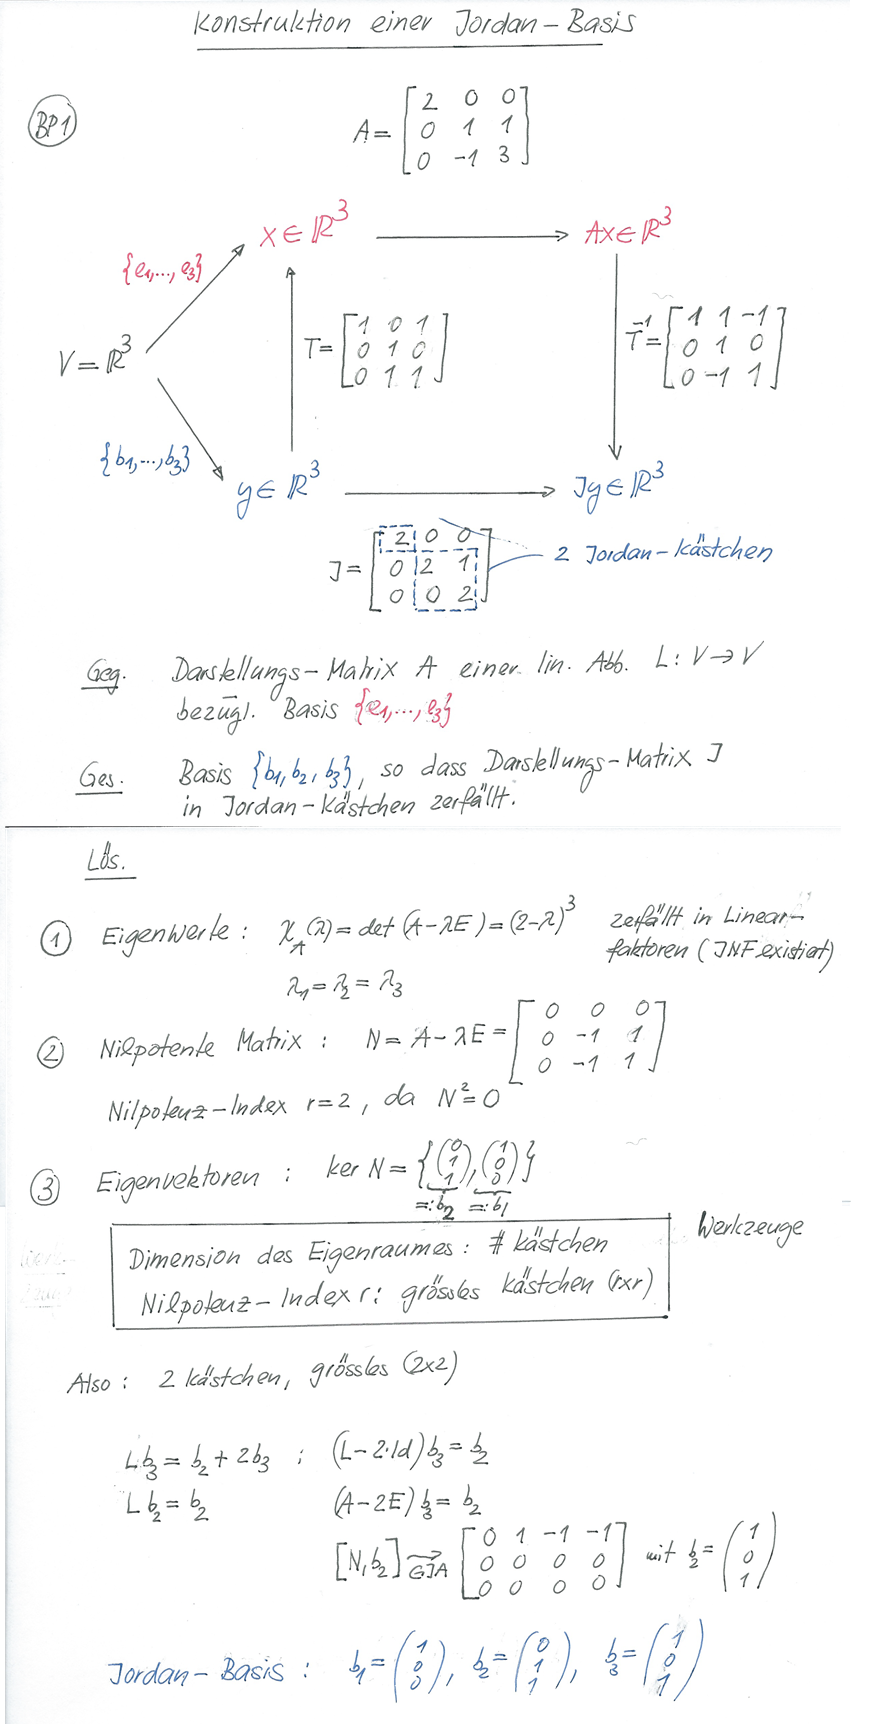
\includegraphics[width=1.0\textwidth]{images/Jordan.png}
%\end{minipage}
%\subsection{Berechnung Jordan Normalform mit TI89}
%Matrix:
%$\begin{bmatrix} %phantom is for spacing
%	2 & \phantom{-}0 & \phantom{-}5\\
%	5 & -3 & \phantom{-}6\\
%	0 & \phantom{-}0 & -3\\
%\end{bmatrix}$
%
%Step 1: Save Matrix\\{}
%[2,0,5;5,-3,6;0,0,-3] $\rightarrow$ a\\
%\hspace*{2cm}$\begin{bmatrix} %phantom is for spacing
%	2 & 0 & 5\\
%	5 & -3 & 6\\
%	0 & 0 & -3\\
%\end{bmatrix}$
%
%Step 2: Eigenwerte\\
%eigVl(a)\\
%\hspace*{2cm} \{-3,2,-3\}
%
%Step 3: Basisvektor $b_1 \rightarrow (A- \lambda_1 I)^n = 0$ für $n=\{1\}$\\
%\textcircled{1} rref(A-2*identity(3))\\
%\hspace*{2cm}$\begin{bmatrix}
%	1 & -1 & 0\\
%	0 & 0 & 1\\
%	0 & 0 & 0\\
%\end{bmatrix}$\\
%
%$\begin{bmatrix}
%	1\;x_1 & -1\;x_2 & 0\;x_3\\
%	0\;x_1 & 0\;x_2 & 1\;x_3\\
%	0\;x_1 & 0\;x_1 & 0\;x_3\\
%\end{bmatrix} = \begin{bmatrix}
%	0\\
%	0\\
%	0\\
%\end{bmatrix} \rightarrow x_1-x_2=0 \; ; \; x_3=0 \rightarrow$ Mögliche Lösung: b1 = $\begin{bmatrix}
%	1\\
%	1\\
%	0\\
%\end{bmatrix}$(da neu, n=max)\\
%
%Step 4: Basisvektor $b_2$ und $b_3 \rightarrow (A- \lambda_2 I)^n = 0$ für $n=\{1,2\}$\\
%\textcircled{2} rref(A+3*identity(3))\\
%\hspace*{2cm}$\begin{bmatrix}
%	1 & 0 & 0\\
%	0 & 0 & 1\\
%	0 & 0 & 0\\
%\end{bmatrix}$\\
%
%$\begin{bmatrix}
%	1\;x_1 & 0\;x_2 & 0\;x_3\\
%	0\;x_1 & 0\;x_2 & 1\;x_3\\
%	0\;x_1 & 0\;x_2 & 0\;x_3\\
%\end{bmatrix} = \begin{bmatrix}
%	0\\
%	0\\
%	0\\
%\end{bmatrix} \rightarrow x_1=0 \; ; \; x_3=0 \rightarrow$ Mögliche Lösung: $\begin{bmatrix}
%	0\\
%	10\\
%	0\\
%\end{bmatrix}$ (Nicht $b_2$, n$\neq$max!!)\\
%
%\textcircled{3} rref((A+3*identity(3))\textasciicircum2)\\
%\hspace*{2cm}$\begin{bmatrix}
%	1 & 0 & 1\\
%	0 & 0 & 0\\
%	0 & 0 & 0\\
%\end{bmatrix}$\\
%
%$\begin{bmatrix}
%	1\;x_1 & 0\;x_2 & 1\;x_3\\
%	0\;x_1 & 0\;x_2 & 0\;x_3\\
%	0\;x_1 & 0\;x_2 & 0\;x_3\\
%\end{bmatrix} = \begin{bmatrix}
%	0\\
%	0\\
%	0\\
%\end{bmatrix} \rightarrow x_1 + x_3=0 \rightarrow$ Mögliche Lösungen: $\begin{bmatrix}
%	0\\
%	1\\
%	0\\
%\end{bmatrix} \; ; \; b3 = \begin{bmatrix}
%	-1\\
%	0\\
%	1\\
%\end{bmatrix}$(da neu, n=max)\\
%
%Step 5: Fehlender Basisvektor $b_2=N_2*b_3$\\
%(A+3*identity(3))*[-1;0;1]\\
%\hspace*{2cm}$\begin{bmatrix}
%	0\\
%	1\\
%	0
%\end{bmatrix}$\\
%
%Step 6: Zusammensetzen
%$T=\begin{bmatrix}
%	b_1 & b_2 & b_3
%\end{bmatrix}$ sowie $J=T^{-1}*A*T$\\{}
%[1,0,-1;1,1,0;0,0,1]$\rightarrow$ t\\
%\hspace*{2cm}$\begin{bmatrix}
%	1 & 0 & -1\\
%	1 & 1 & 0\\
%	0 & 0 & 1\\
%\end{bmatrix}$\\
%t\textasciicircum-1*a*t\\
%\hspace*{2cm}$\begin{bmatrix}
%	2 & 0 & 0\\
%	0 & -3 & 1\\
%	0 & 0 & -3\\
%\end{bmatrix} \rightarrow $ Jordan-Form!

\textbf{Polarkoordinaten}

$\dot{r} = \frac{x\dot{x} + y \dot{y}}{r} \qquad \dot{\Theta} = \frac{x\dot{y} - y\dot{x}}{r^2}$ \\

\textbf{Konservatives Feld/Satz von Poincaré-Bendixson}

Sei $x^*$ ein Fixpunkt eines konservativen dynamischen Systems. Dann ist $x^*$ ein Sattelpunkt oder ein Zentrum. \\ \\
Sei $\dot{x} = f(x)$ ein Vektorfeld in einem beschränkten, abgeschlossenen Teilgebiet $G$ von $\mathbb{R}^2$. Falls $f(x)$ keinen Fixpunkt in $G$ hat und eine Trajektorien $C$ existiert, die ab einer gewissen Zeit $t_0$ für alle $t\in\mathbb{R}$ in $G$ verbleibt, so ist $C$ entweder eine geschlossene Kurve, oder sie konvergiert gegen eine geschlossene Kurve. \\

\textbf{TI NSPIRE CAS}

euler(function, $x$, $f(x)$, \{step begin, step end\}, $f(0)$, h) $ \Rightarrow$ euler($\cos(x/2)$, x, y, \{0, 0.4\}, 0, 0.1)\\ \\

rk23(...)